\documentclass{article}
\usepackage[utf8]{inputenc}

\title{Rover 3 Documentation}
\author{Bobby Stevens}
\date{July 2015}

\usepackage{natbib}
\usepackage{graphicx}
\usepackage{url}
\usepackage{rotating}
\usepackage{multirow}

\begin{document}

\maketitle


\section{Introduction}
Rover is the name designated to the computer in the lab which controls the vacuum pumps and valves for both the Pooh and Tigger chambers. These things are not typically power cycled on a daily basis so their functionality is best contained in an infrequently used computer. Futhermore, these devices need to have interlocks (i.e. automatically be turned off based on some input sensor exceeding a set point) to ensure safe operation.

\subsection{Brief History of Rover}
This is the third incarnation of the Rover machine. The first, and longest running, was built on an Intel 386 based machine and was retired in 2011 after its graphics card failed. Thus ended the ``Good Dog'' era. It was replaced with a Windows XP machine running a LabView program attached to an NI-USB DAQ. This got the job done but had flaws such as requiring a sustained internet connection in order to authenticate LabView. This was the ``Bad Dog'' era. Rover 2 was replaced in 2015 by Rover 3. This marks the beginning of the ``Good Kitty'' era.


\section{Hardware Description}
We have a Raspberry Pi 2 (RP2) computer connected to a custom backplane board that buffers the DIO and provides the A2D chips for measurement by the Pi. The signals for the equipment toggle relays and instrumentation are then sent out to the individual racks for Pooh and Tigger. We will address each of these steps in their own subsection.

\subsection{The Raspberry Pi 2}
Rover 3 is built on a Raspberry Pi 2 model B (RP2). It is running Raspbian (raspberry optimized debian unix) with Gnome 2 installed on top. The RP2 was chosen for its low power consumption (5V @ 1A, max), built in DIO and I2C pins, and more than ample RAM.

Rover 3 interacts with the laboratory equipment through a custom backplane board, see section \ref{sect:backplane}, via its GPIO pins. The pin mapping is shown in figure \ref{fig:gpioPinMapping}. We have purchased a so-called ``cobbler'' board that has a ribbon cable plugged into the GPIO bank and connects to a labeled PCB.

\begin{figure}
\centering
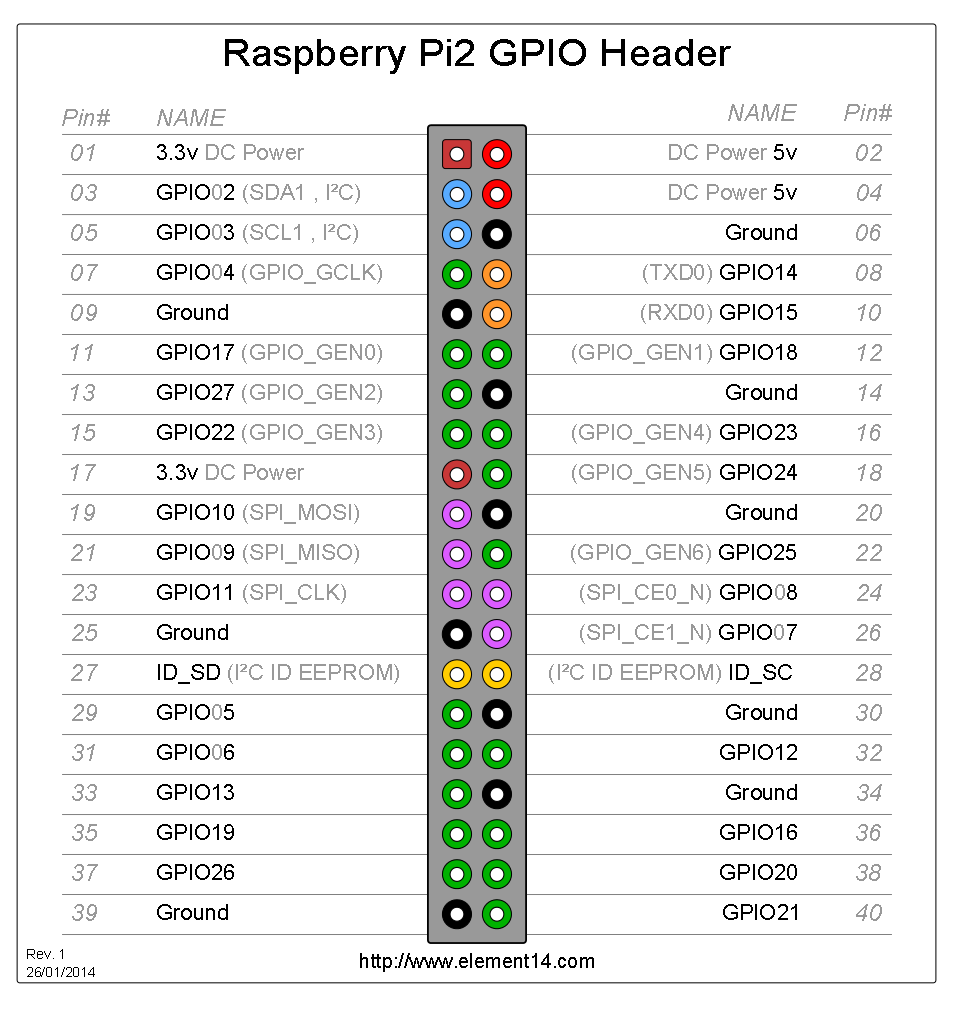
\includegraphics[width=0.9\textwidth]{rp2PinMapping.png}
\caption{A mapping of the GPIO pins on the RP2 board. Interfacing at this level should not be necessary and the same information is printed on the ``cobbler'' board that is mounted to the backplane board. Source: element14.com}
\label{fig:gpioPinMapping}
\end{figure}

The monitor is attached by HDMI. The keyboard and mouse are both USB. Power is provided to the RP2 by a Motorola wall-to-USB transformer (better recognized as a cellphone charger) and plugged into the uninterurptable power supply.


\subsection{The Backplane Board}
\label{sect:backplane}
The RP2 cannot provide enough current on its DIO pins to toggle the relays (16mA max of RP2 compared to .02mA (steady state) and 6mA (switching) for relays). Thus we must buffer these DIO pins if we wish to control multiple relays at once. It also does not have any built-in analog-to-digital converter (ADC) so we will have to provide that functionality and serialize that data in some way. 

The backplane functional diagram is shown in figure \ref{fig:roverBreakout}. An attempt was made to keep the functional diagram and board layout as similar as possible to aid in troubleshooting when the need arises.

\begin{figure}
\centering
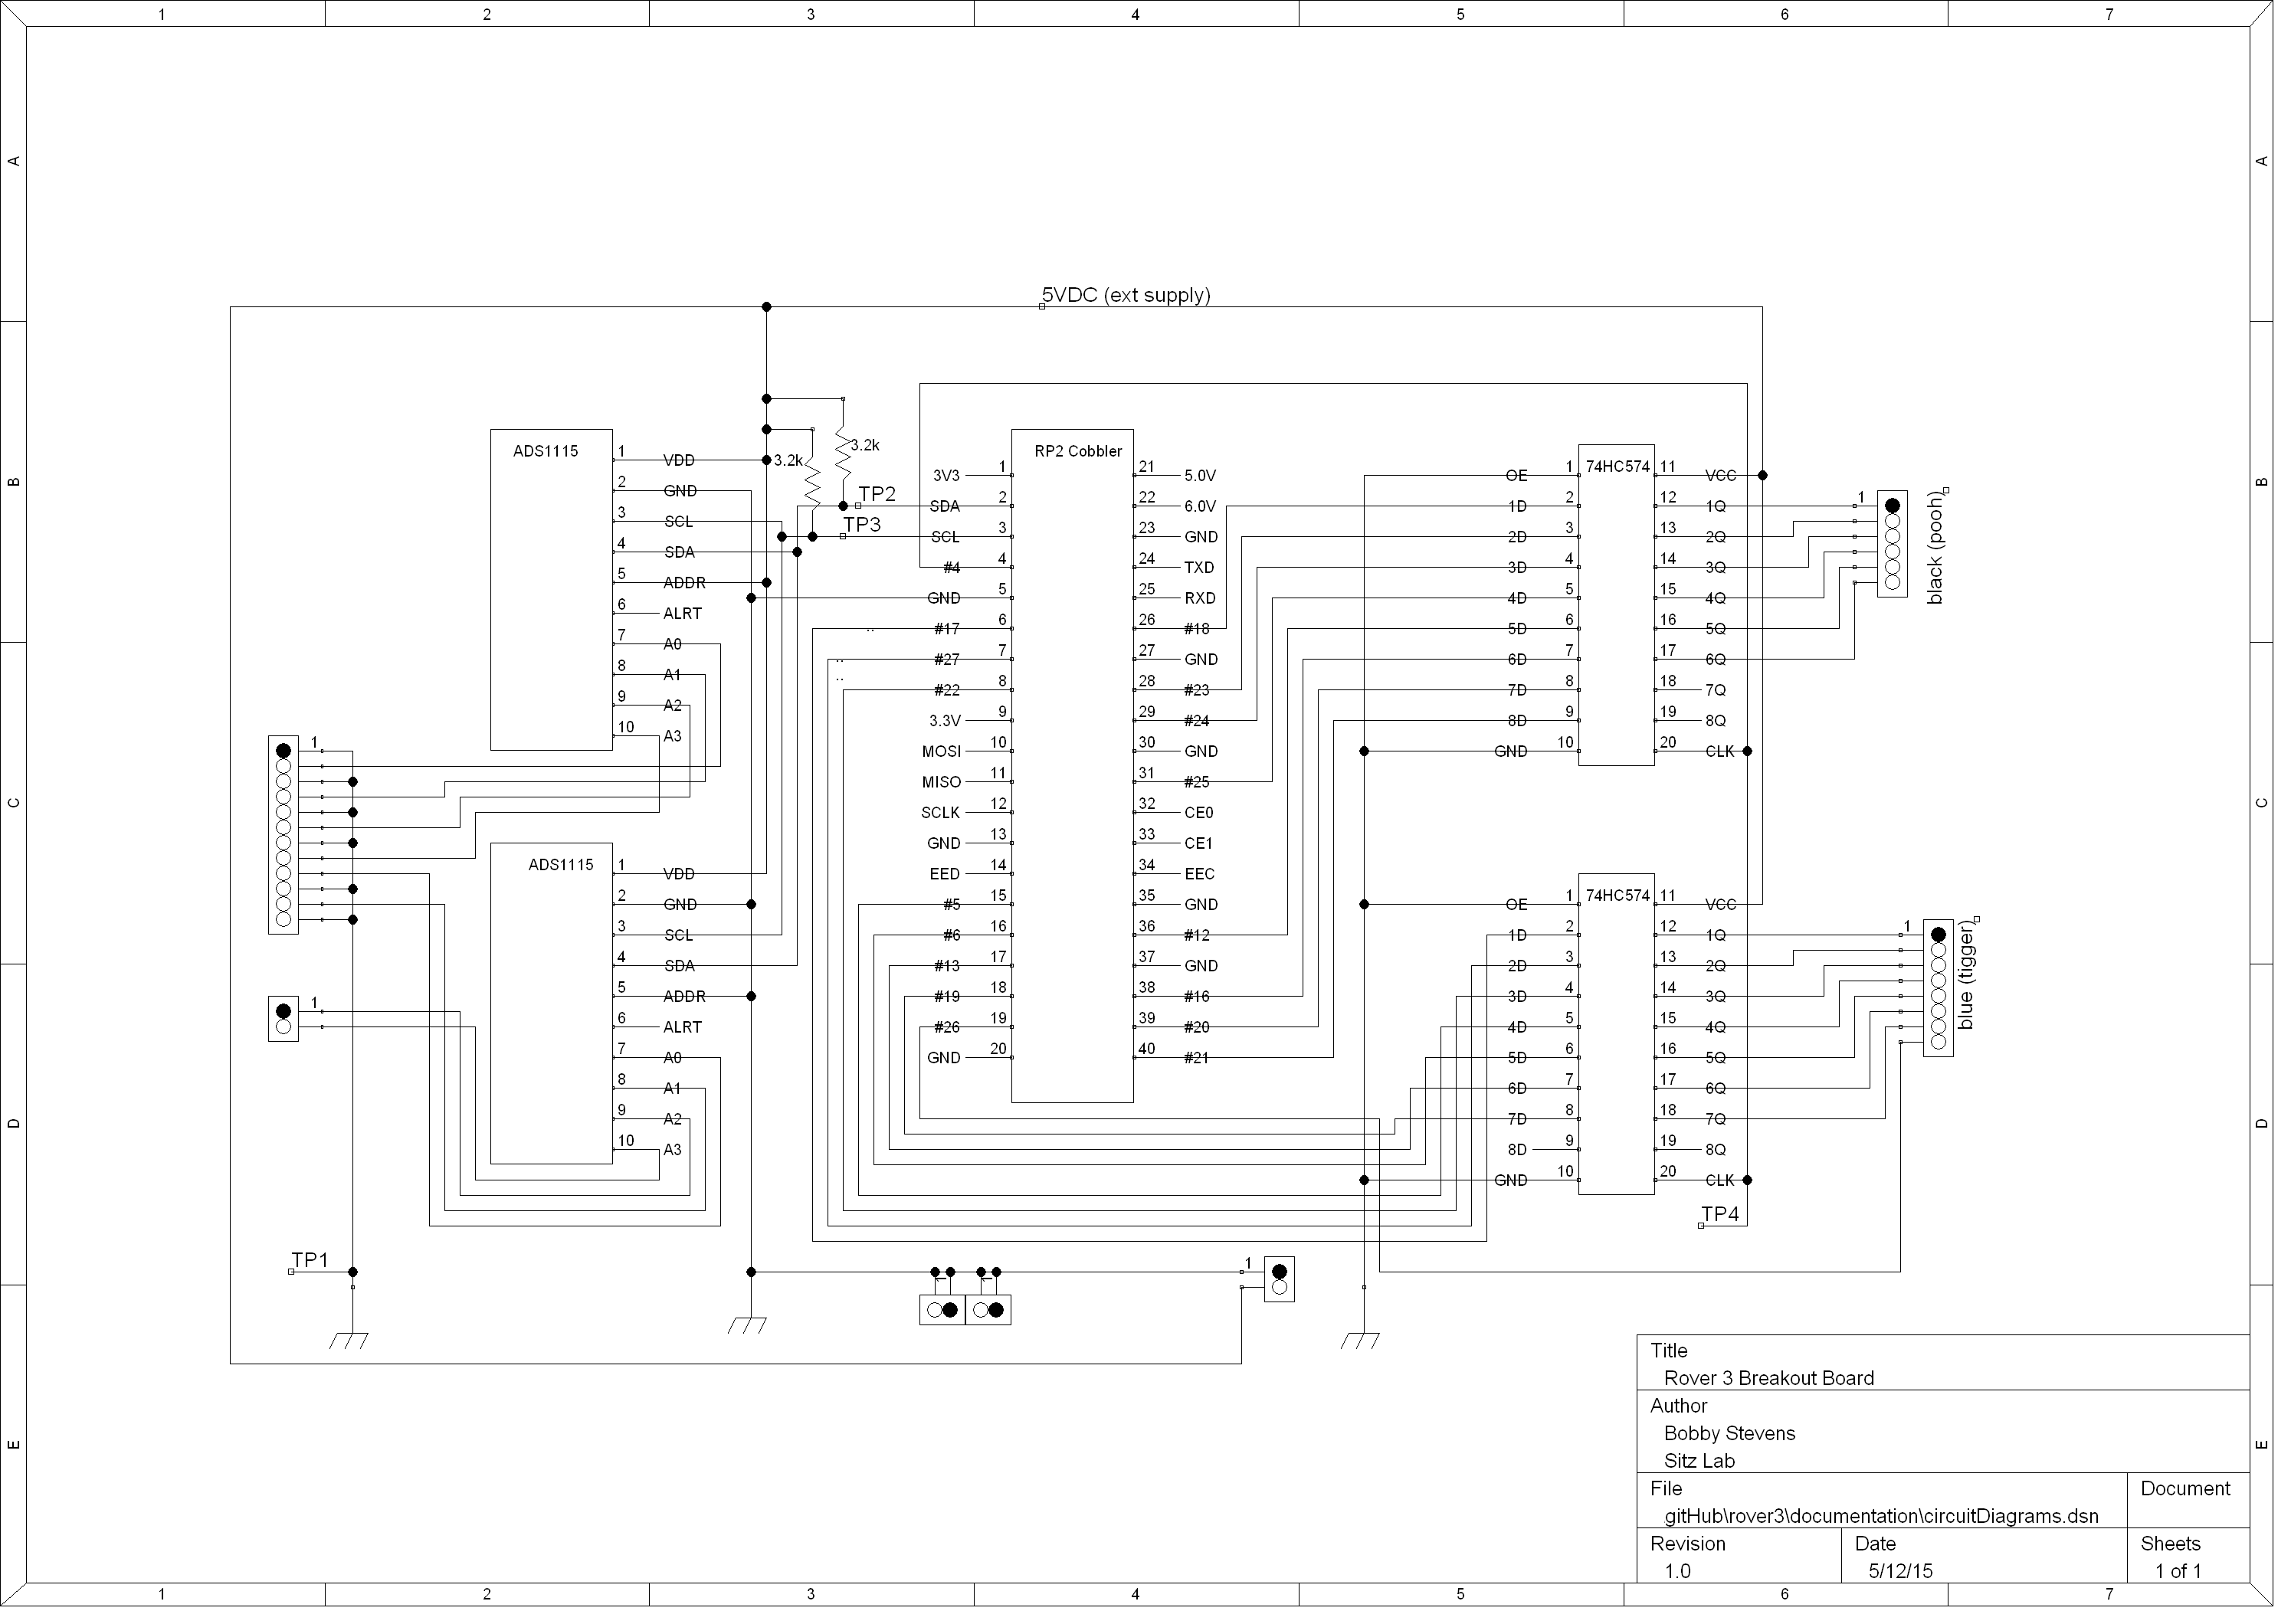
\includegraphics[width=1.5\textwidth, angle = 90]{roverBreakout.png}
\caption{The functional diagram for the RP2 backplane board.}
\label{fig:roverBreakout}
\end{figure}

\subsubsection{DIO Buffering \& Relay Control}
The DIO control is handled on the right side of the backplane board.

A further need for buffering comes from the RP2's DIO reset state on power cycle. When the RP2 is rebooted, its DIO pins get written with an intermediate (TTL) level of 1.5V which is too high to read low and but will be read high by some buffer chips (e.g. 74LS241). This is undesirable because when the RP2 is booting we do not want every piece of equipment to turn on. Thus we use a clockable buffer. The 74HC574 chip has 8 inputs and 8 outputs with a clock pin that will ``write'' the input to the output only on a positive going transition. Thus we design our software (section \ref{sect:software}) to update the proper RP2 DIO pin then use a second DIO pin to clock the buffer thereby pushing that state to the relay or equipment.

The output pins of the 574 are then directly wired to the Pooh (black) and Tigger (blue) screw terminal blocks. The output pin numbers map 1-to-1 with the 574. See figure \ref{fig:roverBreakout}.


\subsubsection{ADC Implementation}
Analog input and digitization is handled on the left side of the backplane board, see figures \ref{fig:roverBreakout} and \ref{fig:roverBreakoutPicTop}.

As previously mentioned, the RP2 does not have any built-in ADC. We have 7 analog inputs that we need to interlock based upon their values. All but one of these needs to be a referenced single-ended (RSE) termination style which will require 6 ADCs. The remaining analog input needs to be measured in differential mode thus requiring 2 ADCs of its own. Thus we need 8 ADCs.

We will never need to respond very quickly to changes on any of these inputs. A response time of a few seconds is more than enough to establish safety with the diffusion pumps which take approximately 45 minutes to cool down anyways. Thus we do not need particularly fast ADCs.

Based on these requirements we can easily get by with a multiplexed ADC (multiple inputs are measured by 1 ADC in serial). TI's ADS1115 is precisely what we need. It has 4 inputs that will be multiplexed to a 16-bit 860SPS ADC. This information will be communicated by the I2C (or $I^2C$) interface. 

I2C is a serialized data communication protocol. This is done over two wires: a data wire (SDA) and a clock wire (SCL). Devices can only pull these wires low so a pull-up resistor is required to improve the time response (resistors R1 and R2 in figure \ref{fig:roverBreakout}). As in other protocols, there is a master and multiple slaves. For I2C each slave has a programmable 7-bit address. In the case of the ADS1115 the address pin will be tied low to make the address be 0x63 or tied high to make the address be 0x64. A key distinction for I2C is that any device can assert the clock pin low. This is important if you wish to truly understand how the communication works.

A timeline of how I2C works follows, refer to figure \ref{fig:i2cTiming} while reading. The master will send on SDA an address that it wants to either read or write from followed by a read/write bit. If that device is powered and on the lines it will respond the next clock cycle with the acknowledge or ``ack'' bit. Messages are limited to 8bits. If a read is specified the slave will load its data onto the SDA and clock SCL. If a write is specified the master will load data onto SDA and clock SCL. For more information on I2C see Horowitz and Hill.

\begin{figure}
\centering
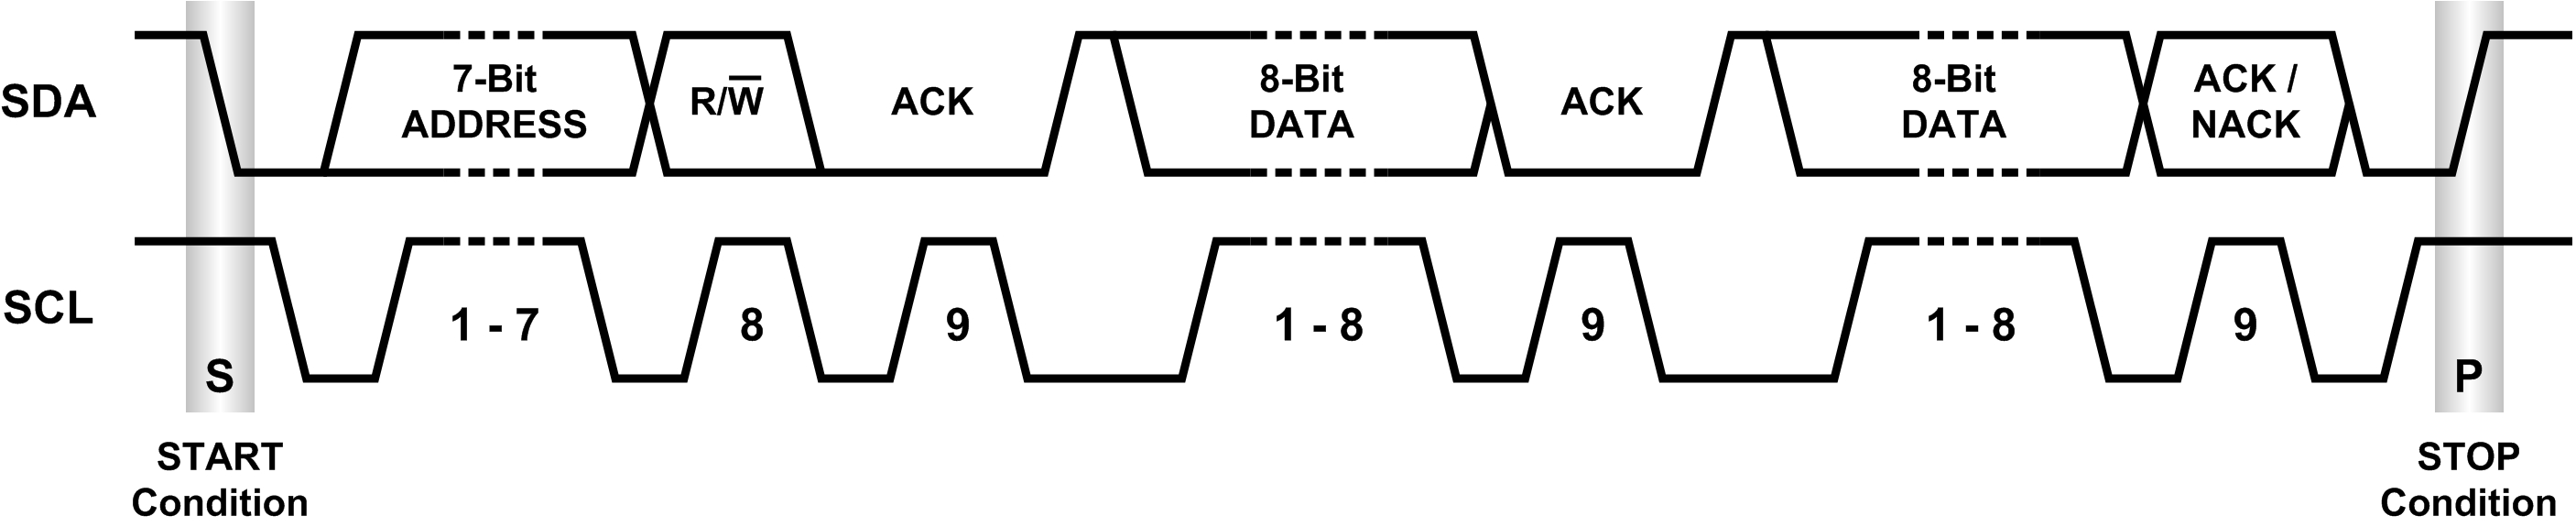
\includegraphics[width=0.9\textwidth]{i2cTiming.png}
\caption{A timing diagram showing how I2C communication works. Source: cmpnet.com}
\label{fig:i2cTiming}
\end{figure}

To present the 4 inputs of the ADS1115 to the user each input is wired into a screw terminal and the adjacent terminal is connected to ground. This will allow you to connect RSE inputs by wiring into two adjacent terminals or differential by wiring into one terminal, skipping a terminal (ground), and wiring into the next. Be aware that if you need to measure differential you will have to reconfigure the input in software (see section \ref{sect:software}). There are two screw terminals on the AI side that are separated from the rest. These are the differential inputs that are wired into A2 and A3 on ADS1115-B.


\subsubsection{Wiring \& Test Points}
There was significant effort in making the wires color coded. The meanings for each color are listed in this table.

\begin{table}[h]
\begin{tabular}{r|l}
Wire Color & Function \\ \hline
Red & +5VDC \\ \hline
Black & Ground \\ \hline
Purple & clocking pin for 574 chips \\ \hline
Orange & I2C clock \\ \hline
Green & I2C data \\ \hline
Yellow, White, Lime Green, Blue & data lines, patterned in that order. \\
\end{tabular}
\end{table}

The test points are listed here:

\begin{table}[h]
\begin{tabular}{r|l}
Test Point (Color) & Function \\ \hline
TP0 (Black) & Ground  \\ \hline
TP1 (Purple) & DO clock \\ \hline
TP2 (Lime Green) & I2C clock \\ \hline
TP3 (Blue) & I2C data \\ 
\end{tabular}
\end{table}


\subsection{24VDC Relays Board}
This ancillary board should be viewed as a 24VDC ``booster'' to the 5VDC DIO lines from the 574. 4 pieces of equipment (Pooh gate valve, Pooh foreline valve, Tigger source foreline valve, and Tigger main foreline valve) need 24VDC to switch. It also contains a voltage divider on the 24V supply for a power sense line so that Rover can execute a power failure routine. The boosting is done with 4 Gordos 831A relays (datasheet included). 

\begin{figure}
\centering
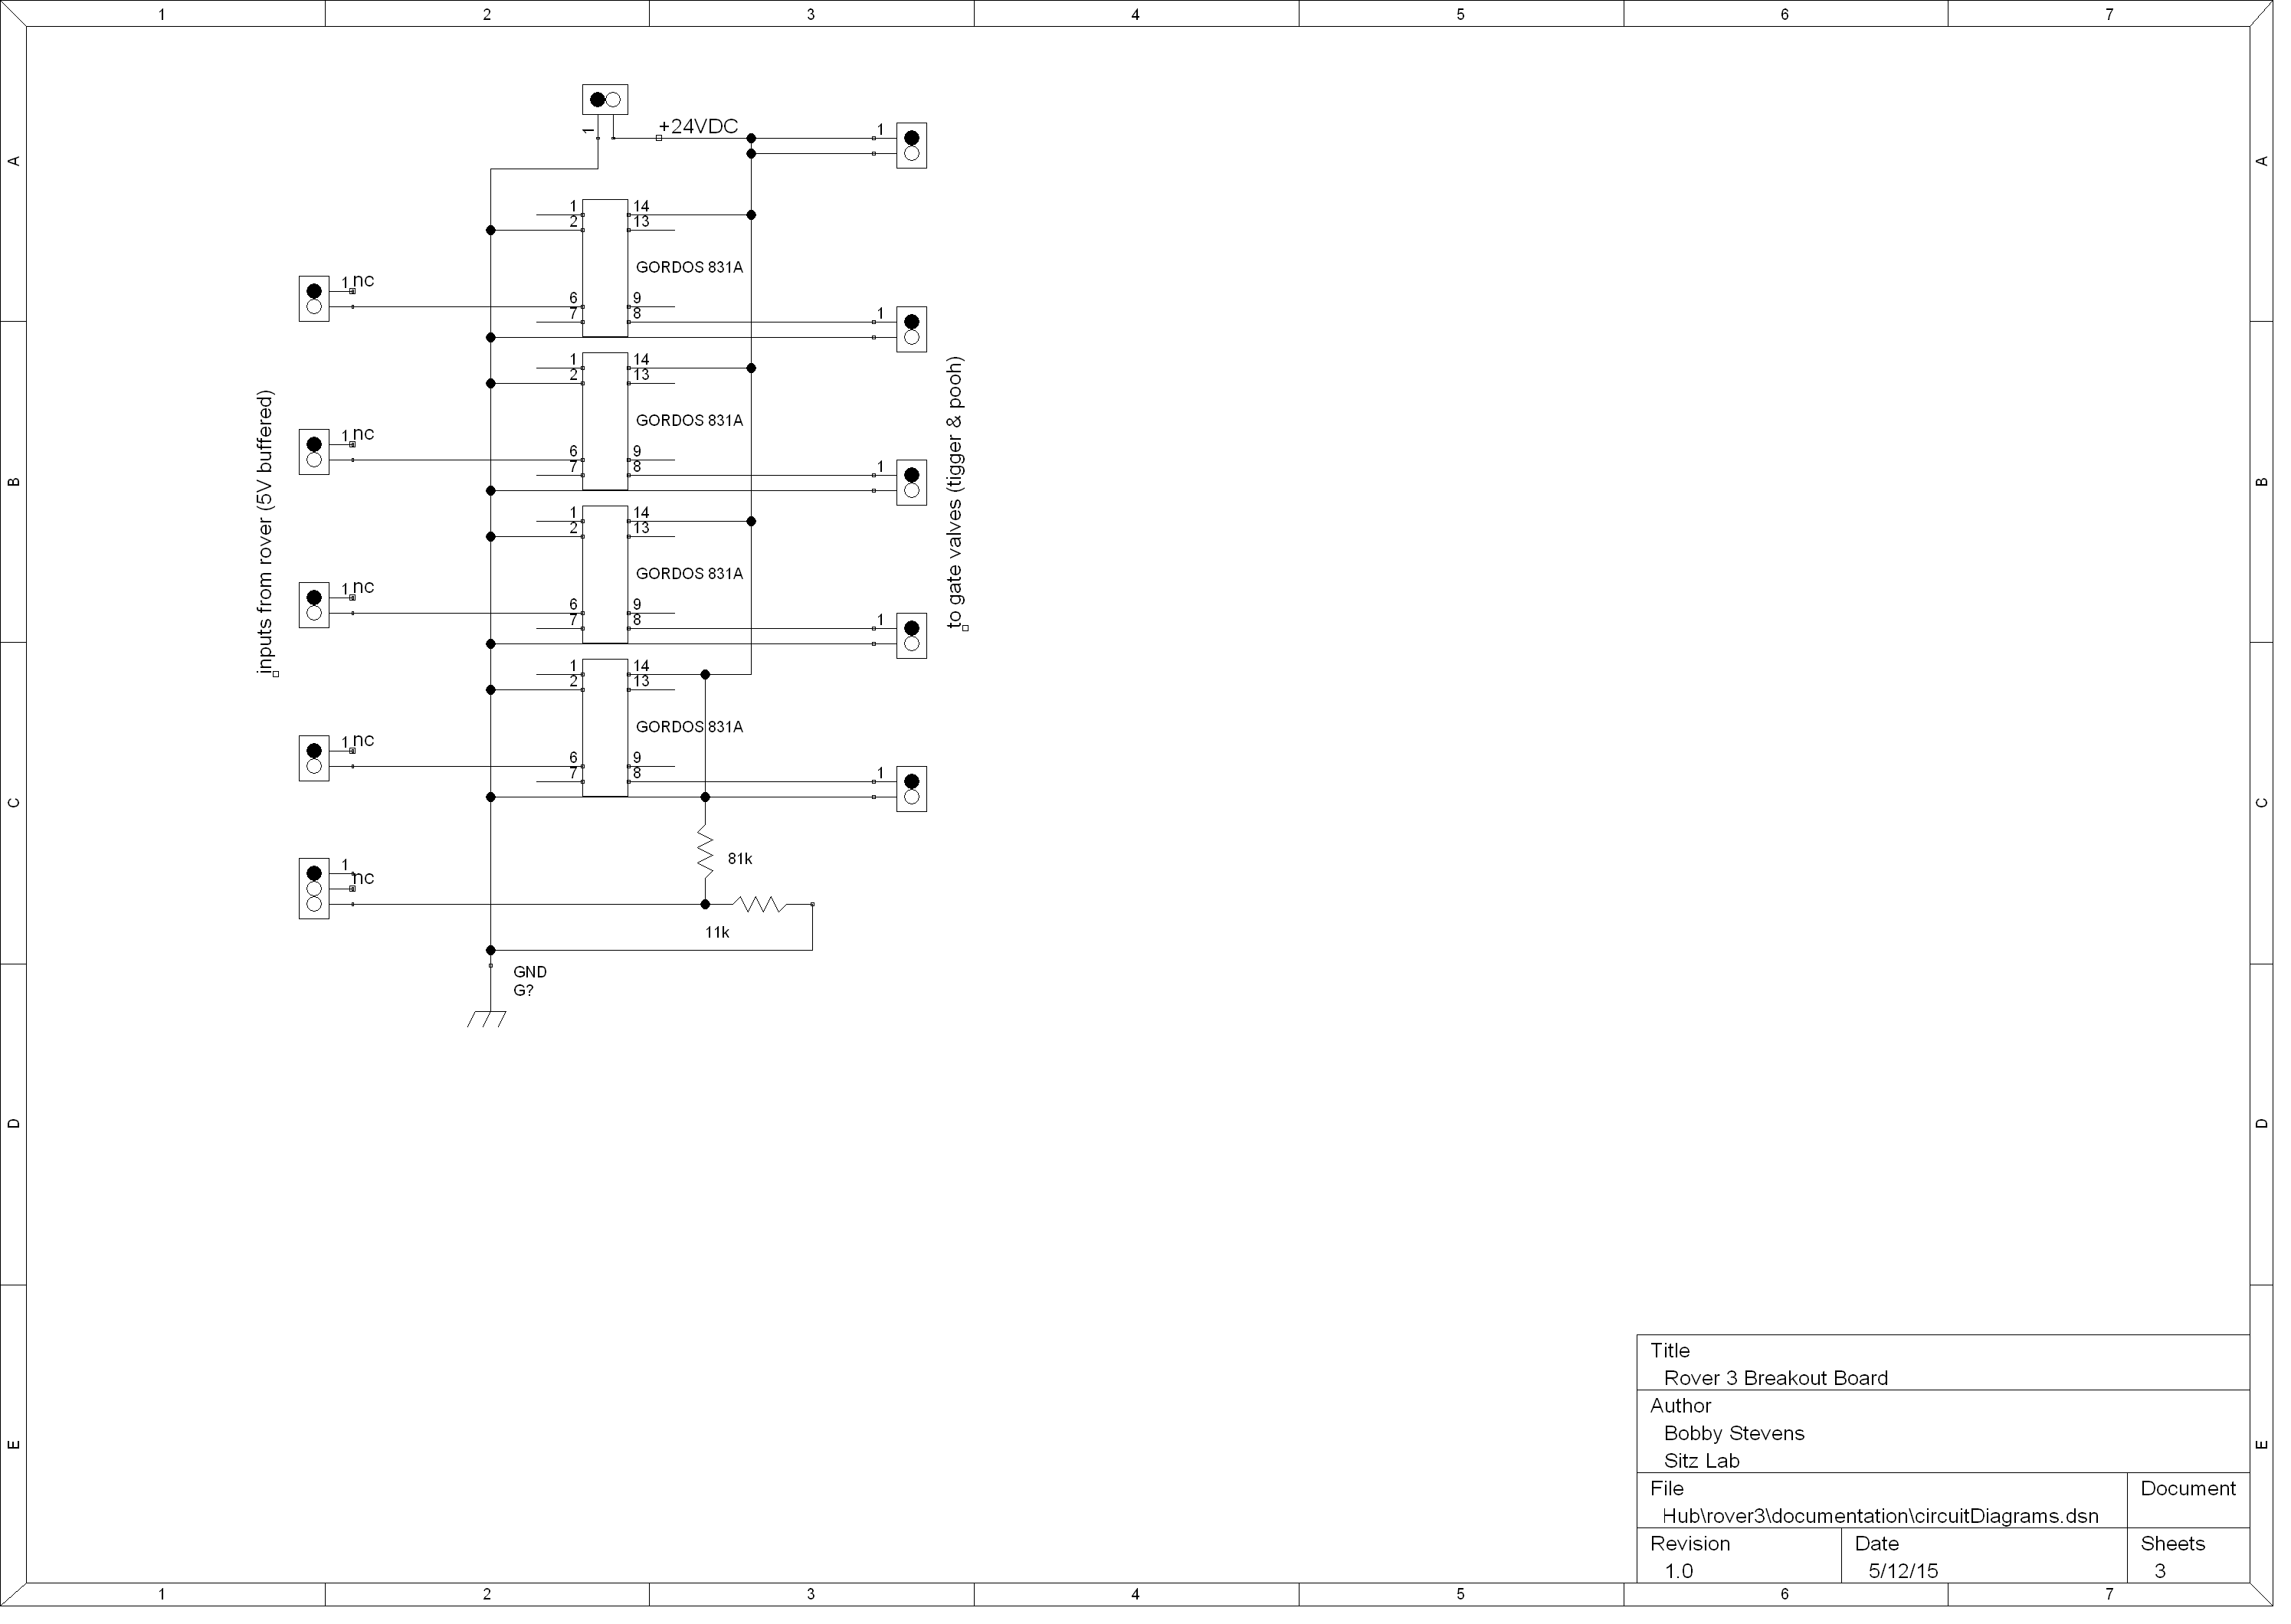
\includegraphics[width=0.9\textwidth]{24VDCBreakout.png}
\caption{The functional diagram for the 24VDC relays board.}
\label{fig:24VDCBreakout}
\end{figure}


\subsection{120VAC Relays Board}
This is another ancillary board to switch 120VAC for 2 pieces of equipment on Tigger: the buffer and main gate valves. These are Crydom D2W solid state relays which take wall voltage input and connect the hot line to common through the equipment. The datasheet for these is included.

\begin{figure}
\centering
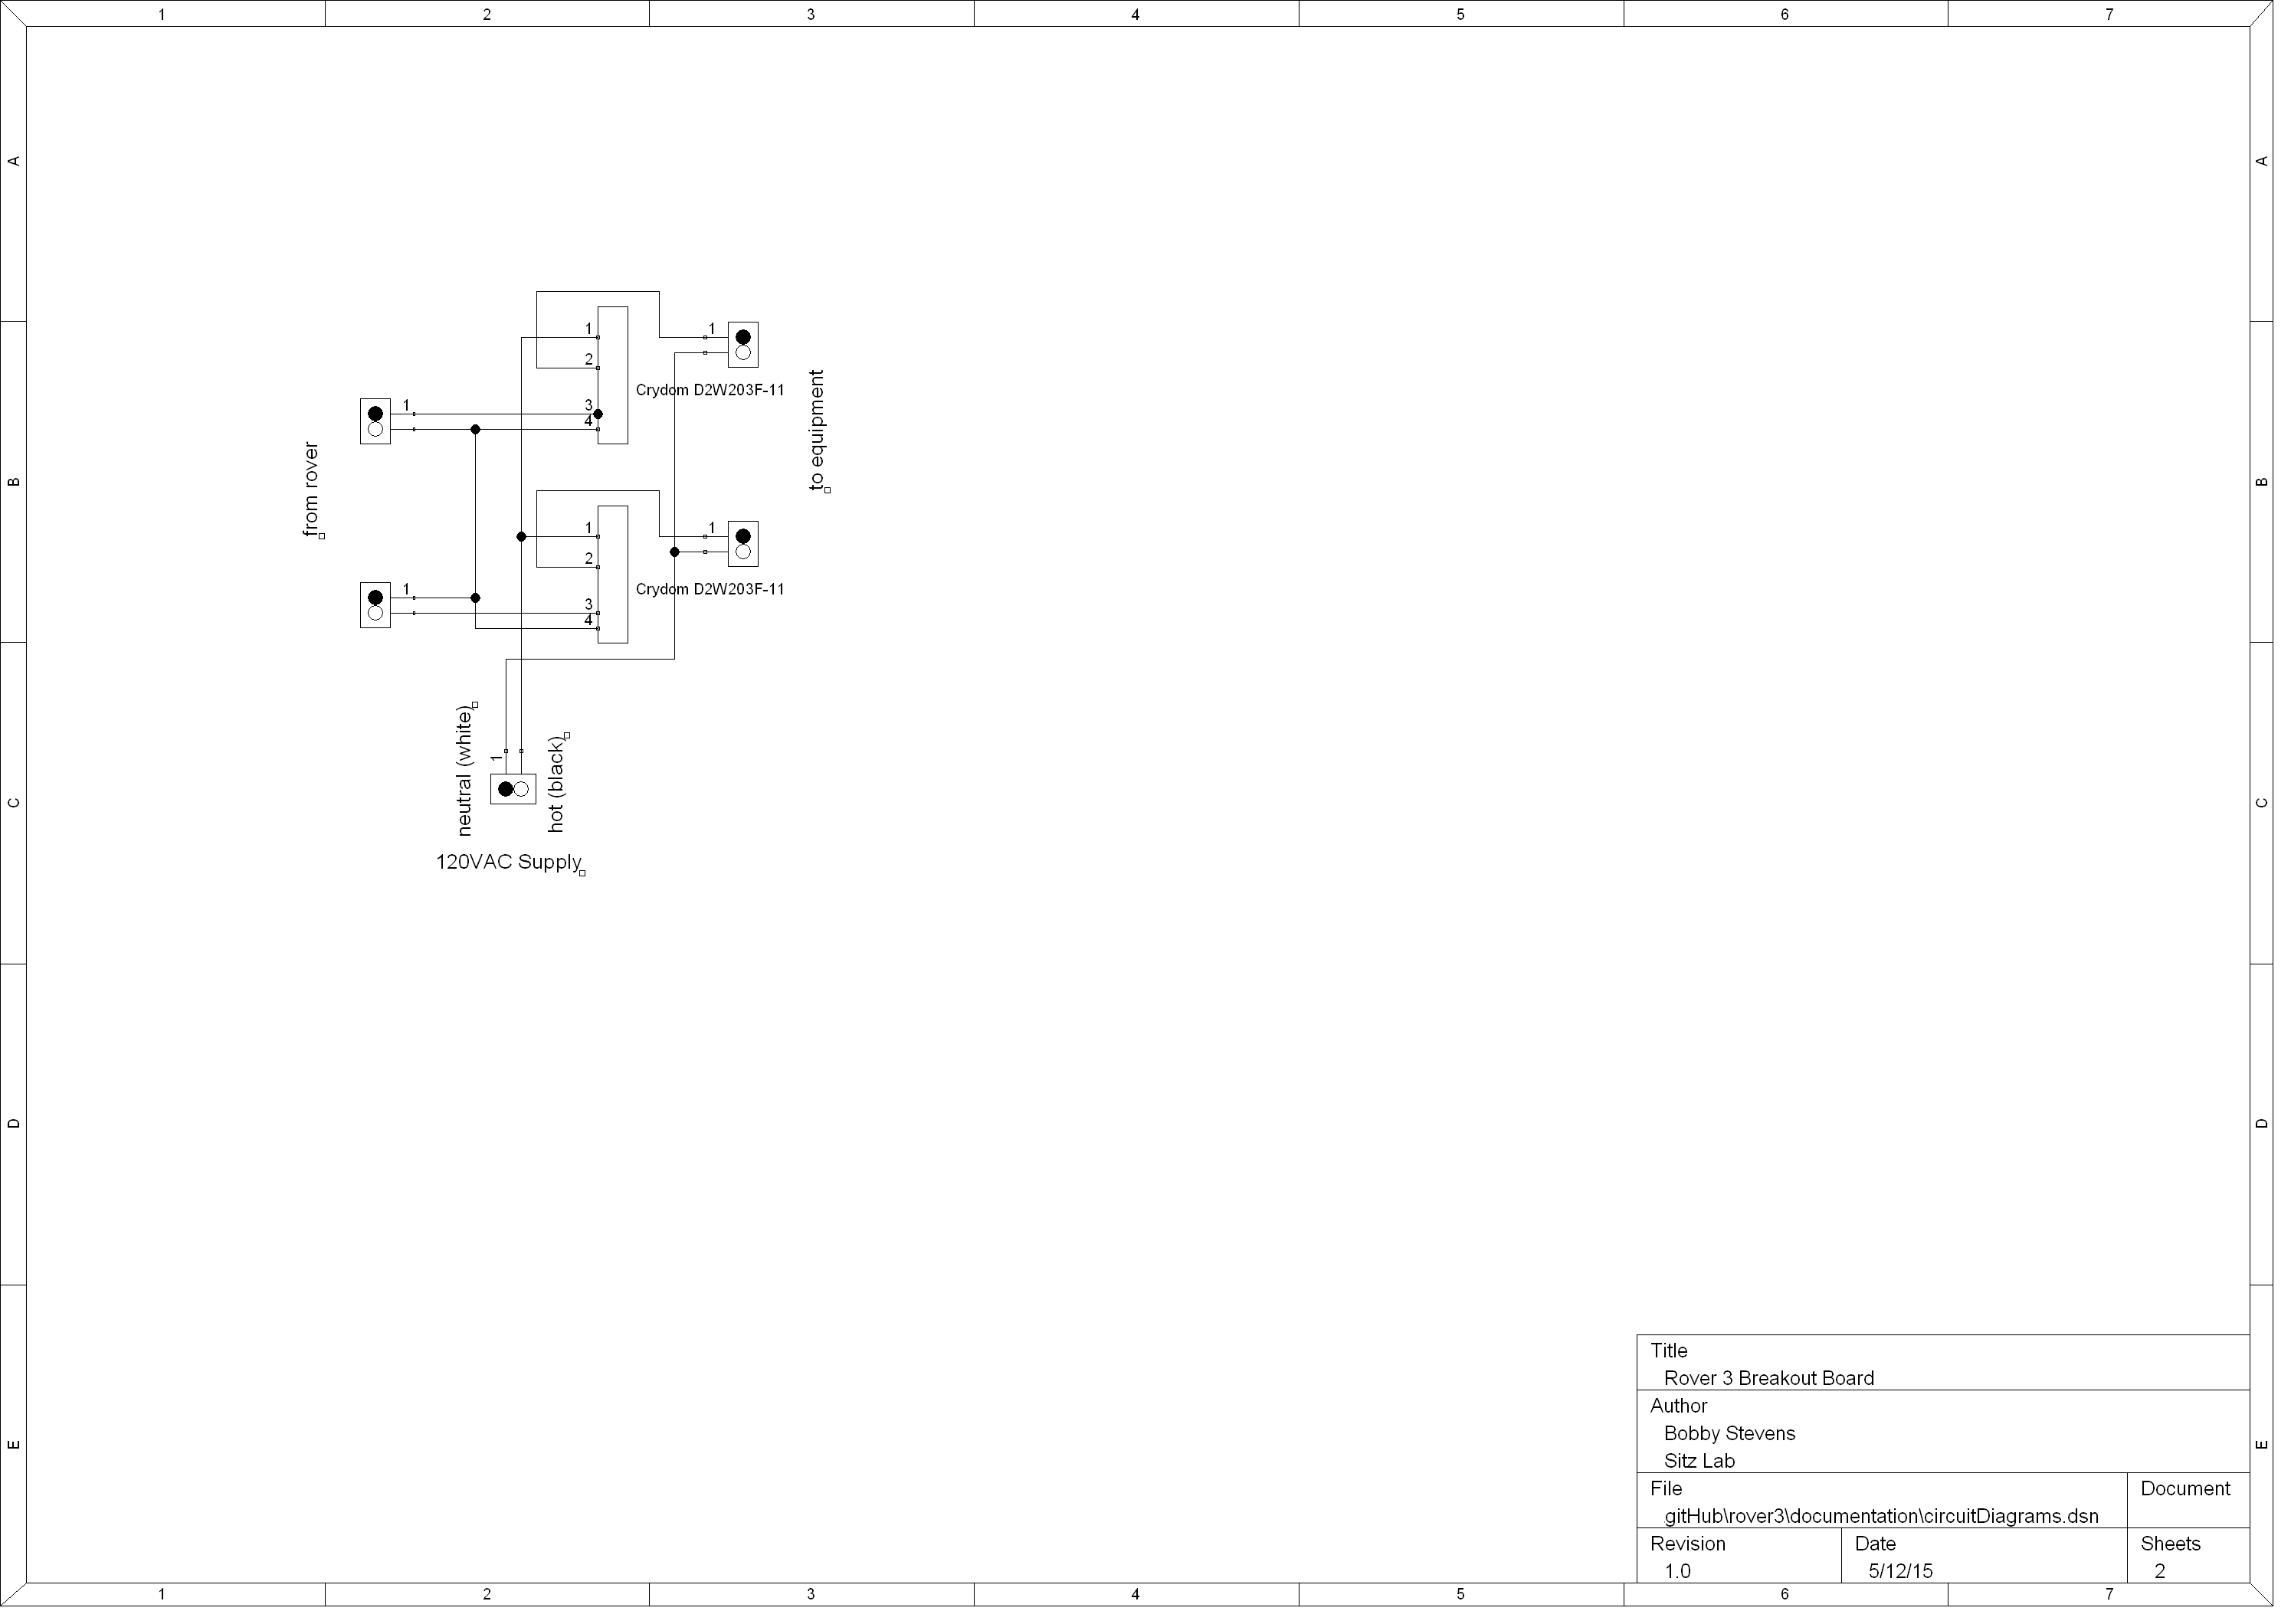
\includegraphics[width=0.9\textwidth]{120VACBreakout.png}
\caption{The functional diagram for the 120VAC relays board.}
\label{fig:120VACBreakout}
\end{figure}






\section{Software Description}
\label{sect:software}
The software package for Rover 3 is available at \texttt{https://github.com/stevens4} \texttt{/rover3.git}. It is written in Python. The main program, \texttt{roverServer.py}, needs superuser permissions to access the DIO pins so it needs to be run as such, i.e. \texttt{sudo  python  roverServer.py}. An attempt was made to write the code in as modular a style as possible. From here we will discuss each module in turn.

\subsection{Standard Libraries}
The Rover 3 software requires 4 free-to-use libraries in order to run. Some of these libraries will need to be installed separately while others exist within the Github project. Here we will briefly state the function of each library within the project.

\noindent
\textbf{\emph{PySide:}} this is the GUI library used. It is a large project that maps the C++ QT framework to a python version. \textbf{Must be installed separately.}

\noindent
\textbf{\emph{RPi GPIO:}} allows control of the DIO pins from within python. \textbf{Must be installed separately.}

\noindent
\textbf{\emph{Adafruit ADS1x15:}} allows for interfacing with the ADS1115 chips within I2C protocol. \textbf{Bundled into project.}

\noindent
\textbf{\emph{Adafruit I2C:}} required for the Adafruit ADS1x15 library. \textbf{Bundled into project.}


\subsection{Custom Libraries}
The following libraries are files that were written by the author and are considered part of this project. They are libraries only in the sense that they are not executable on their own. We will spend a bit more time explaining these two libraries since customization will most likely take place at this level.


\subsubsection{\texttt{lowLevelLibrary.py}}
This library defines the hardware chips as software objects. It defines the \texttt{aiChannel}, \texttt{doChannel}, and \texttt{interlock} objects. The methods provided in each object should allow for any operations or configurations that are needed.

AIChannel objects can be configured only on initialization and will provide a mapped value based on the voltage that was previously measured. This mapping function is defined in the config, see section \ref{sect:config}, for each channel.

DOChannel objects have a specified RP2 pin they can toggle and a ``clock function'' they execute when a toggle is executed. The clock function is normally used to cycle the clock pin of the 574 chips. DOChannels can be toggled or polled for their current state and have a list of interlocks that can be reconfigured, added to, or removed from.

Interlock objects are owned by a DOChannel. An interlock is simply a logical statement concerning an AIChannel and a set point. \textbf{When this logical statement is \emph{true} the interlock will trip and turn the DOObject off.} Interlocks can be set from within the roverServer interface and are saved to a config directory to persist after the GUI is closed. 


\subsubsection{\texttt{customWidgets.py}}
This is the higher level library that defines customized PySide objects for the roverServer GUI with extended functionality to interface with hardware. It defines the \texttt{doControlRow} and \texttt{interlockConfig} objects.

\texttt{doControlRow} is a widget (see PySide documentation for terminology) that has the LED indicator, power toggle button, device label, interlock config button, and interlock override button. Each doObject has an associated doControlRow. The LED indicator comes from the SitzLabExpControl project but a copy is bundled into this package. 

\texttt{interlockConfig} is a dialog summoned from the doControlRow's interlock config button. This dialog allows the user to view and modify existing interlocks, remove interlocks, and add new interlocks. When the dialog is confirmed the interlocks are written to a config file and immediately take effect for this doControl object.


\subsubsection{\texttt{config.py}}
\label{sect:config}
The config file contains a dictionary of dictionaries for the analog inputs and digital outputs. This is where you can edit the GUI location and label text for both AIObjects and DOObjects and change which physical channels each are associated with. The AIChannels also have amplification factors for the ADC chip, the read rate, and the mapping function. The mapping function can either be ``poly'' (polynomial up to order 4) or ``exp'' (exponential). These functions will be applied to new measured voltages before they are sent to the GUI to be displayed as a value with units (e.g. pressure in milliTorr).


\subsection{Rover Server}
Rover server is mostly the GUI commands to initialize the environment. Most of this code will not need to be changed unless aesthetics are of concern. Key parts of the code that are not for GUI creation include the digital output clocking function \texttt{cycleDOClock()} and the A2D polling thread object \texttt{A2DThread()}. These are higher level functions that interface with the low level hardware and must be at the top level of code to ensure either (a) each DO toggle clocks the write pin or (b) each analog input is read in serial and conflicting calls are not made concurrently.


\section{Physical Connections}
Here we provide two tables for the controls (outputs of Rover) table \ref{tab:controls} and sensors (inputs to Rover) table \ref{tab:sense}. This information is also presented in figure \ref{fig:wiringDiagram}. Figure \ref{fig:roverOverhead} is a picture of the Rover system with helpful definitions of screw terminal labels.

\begin{figure}
\centering
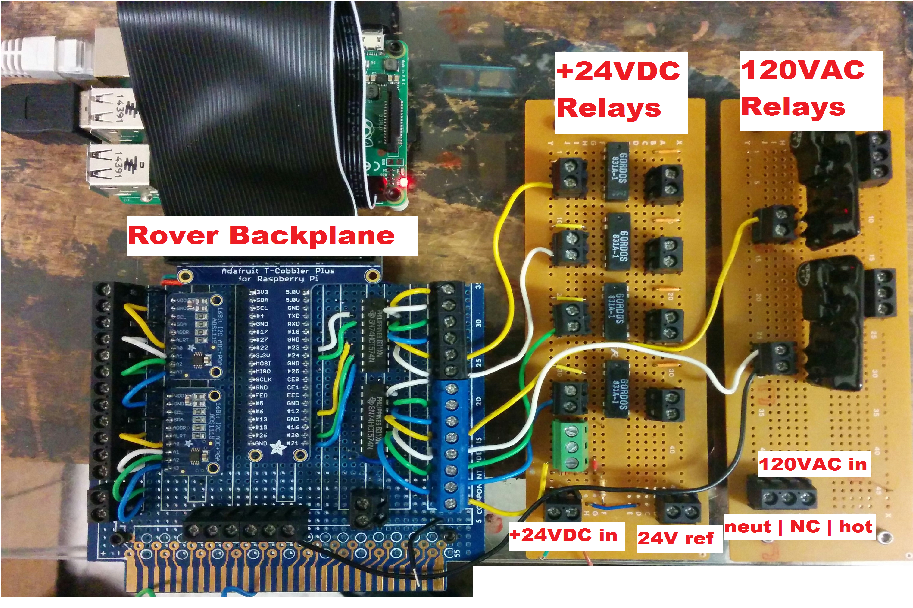
\includegraphics[width=0.9\textwidth]{roverOverhead.png}
\caption{Labeled components of the hardware interface. The backplane board is more detailed in figure \ref{fig:roverOverhead2}. The ancillary 24VDC and 120VAC boards are labeled and their supply terminals marked.}
\label{fig:roverOverhead}
\end{figure}

\begin{figure}
\centering
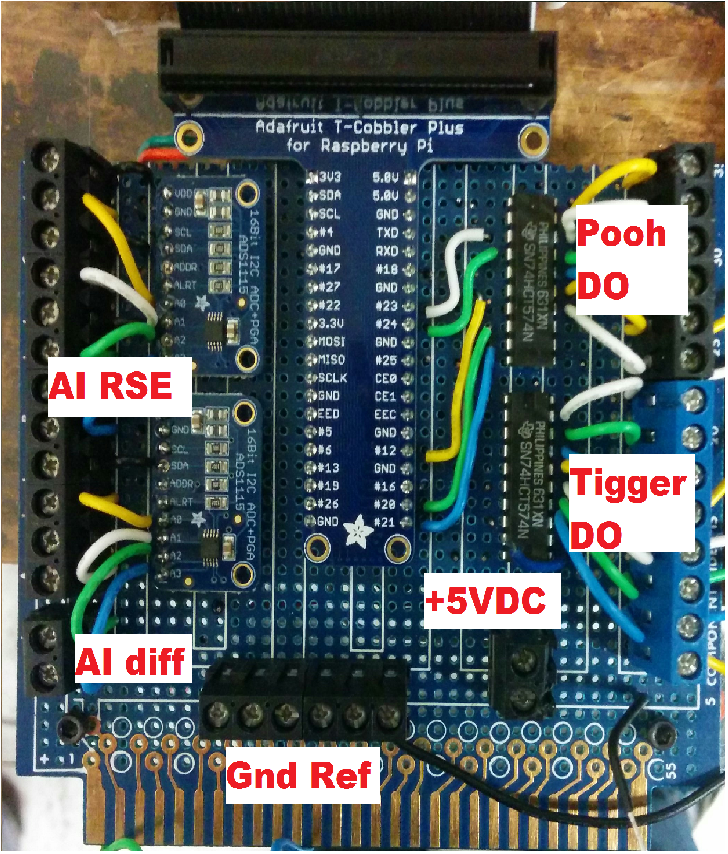
\includegraphics[width=0.9\textwidth]{roverOverhead2.png}
\caption{Labeled components of the rover backplane board. On the left are the analog inputs and on the right are the digial outputs. The 12 unit long black screw terminal on the left are the AI RSE with every odd terminal connected to ground (note black wire indicating ground). The separate 2 unit terminal below is the AI differential input. The 6 unit black on the bottom are ground reference connections for the Pooh and Tigger devices, see table \ref{tab:controls}. The 2 unit black next to that is the +5VDC supply for the backplane components; both the ADS1115 and 574 chips are powered through this. The 6 unit black terminal on the right are the Pooh digital outputs. The 8 unit blue terminal is for Tigger with the exception being last position which is the lab power sense input that is connected to the green block on the +24VDC board.}
\label{fig:roverOverhead2}
\end{figure}


\begin{table}[]
\centering
\caption{the sensor connections for the Rover system}
\begin{tabular}{c|r|r|r|r}
& Label & ADS1115 pin & Screw Terminal & Wire ID \\ \hline
\multirow{2}{*}{pooh} & main foreline pressure & A0 & A1-2 & ?? \\ \cline{2-5}
& source foreline pressure & A1 & A3-4 & ?? \\ \hline \hline
\multirow{3}{*}{tigger} & main foreline pressure & A2 & A7-8 & ?? \\ \cline{2-5}
& source foreline pressure & B0 & A9-10 &  ?? \\ \cline{2-5}
& buffer foreline pressure & B1 & A11-12 & ?? \\ \hline \hline
both & water temp & B2-3 & B1-2 & \\ \cline{2-5}
& spare RSE & A3 & A5-6 & N/A
\end{tabular}
\label{tab:sense}
\end{table}



\begin{sidewaystable}[]
\centering
\caption{the control connections for the Rover system}
\begin{tabular}{c|r|r|r|r|r|r}
\parbox[t]{2mm}{\multirow{8}{*}{\rotatebox[origin=c]{90}{pooh}}} & Label & RP2 Pin & 574 Pin & Screw Terminal & Buffer Chip & Wire Color \\ \cline{2-7}
 & +5VDC reference & N/A & N/A & ?? & N/A & orange \\ \cline{2-7}
 & +24VDC reference & N/A & N/A & ?? & N/A & white \\ \cline{2-7}
 & +24VDC reference & N/A & N/A & ?? & N/A & white-black \\ \cline{2-7}
 & water valve & 18 & A1 & Black 1 & N/A & yellow \\ \cline{2-7}
 & main roughing pumps & 23 & A2 & Black 2 & N/A & black \\ \cline{2-7}
 & source roughing pumps & 24 & A3 & Black 3 & N/A & blue \\ \cline{2-7}
 & source diffusion pumps & 25 & A4 & Black 4 & N/A & brown \\ \cline{2-7}
 & main gate valve & 12 & A5 & Black 5 & Gordos-1 & purple \\ \cline{2-7}
 & main foreline valve & 16 & A6 & Black 6 & Gordos-2 & grey \\ \hline \hline
 & gnd reference & N/A & N/A & ?? & N/A & red \\ \cline{2-7}
\parbox[t]{2mm}{\multirow{7}{*}{\rotatebox[origin=c]{90}{tigger}}} & spare & 17 & B1 & Blue 1 & N/A & N/A \\ \cline{2-7}
 & water valve & 27 & B2 & Blue 2 & N/A & green \\ \cline{2-7}
 & diffusion pumps & 22 & B3 & Blue 3 & N/A & brown, blue, yellow, orange \\ \cline{2-7}
 & buffer foreline valve & 5 & B4 & Blue 4 & Crydom-1 & dark grey \\ \cline{2-7}
 & main gate valve & 6 & B5 & Blue 5 & Crydom-2 & white \\ \cline{2-7}
 & source foreline valve & 13 & B6 & Blue 6 & Gordos-3 & white-red \\ \cline{2-7}
 & main foreline valve & 19 & B7 & Blue 7 & Gordos-4 & white-green \\ \cline{2-7}
 & gnd reference & N/A & N/A & ?? & N/A & white-black \\ \cline{2-7}
 & gnd reference & N/A & N/A & ?? & N/A & white-white \\ \cline{2-7}
 & gnd reference & N/A & N/A & ?? & N/A & green \\ \hline \hline
\parbox[t]{2mm}{\multirow{3}{*}{\rotatebox[origin=c]{90}{general}}} & power sense & 26 & N/A & Blue 8 & 24VDC divide & N/A  \\ \cline{2-7}
\end{tabular}
\label{tab:controls}
\end{sidewaystable}


\begin{figure}
\centering
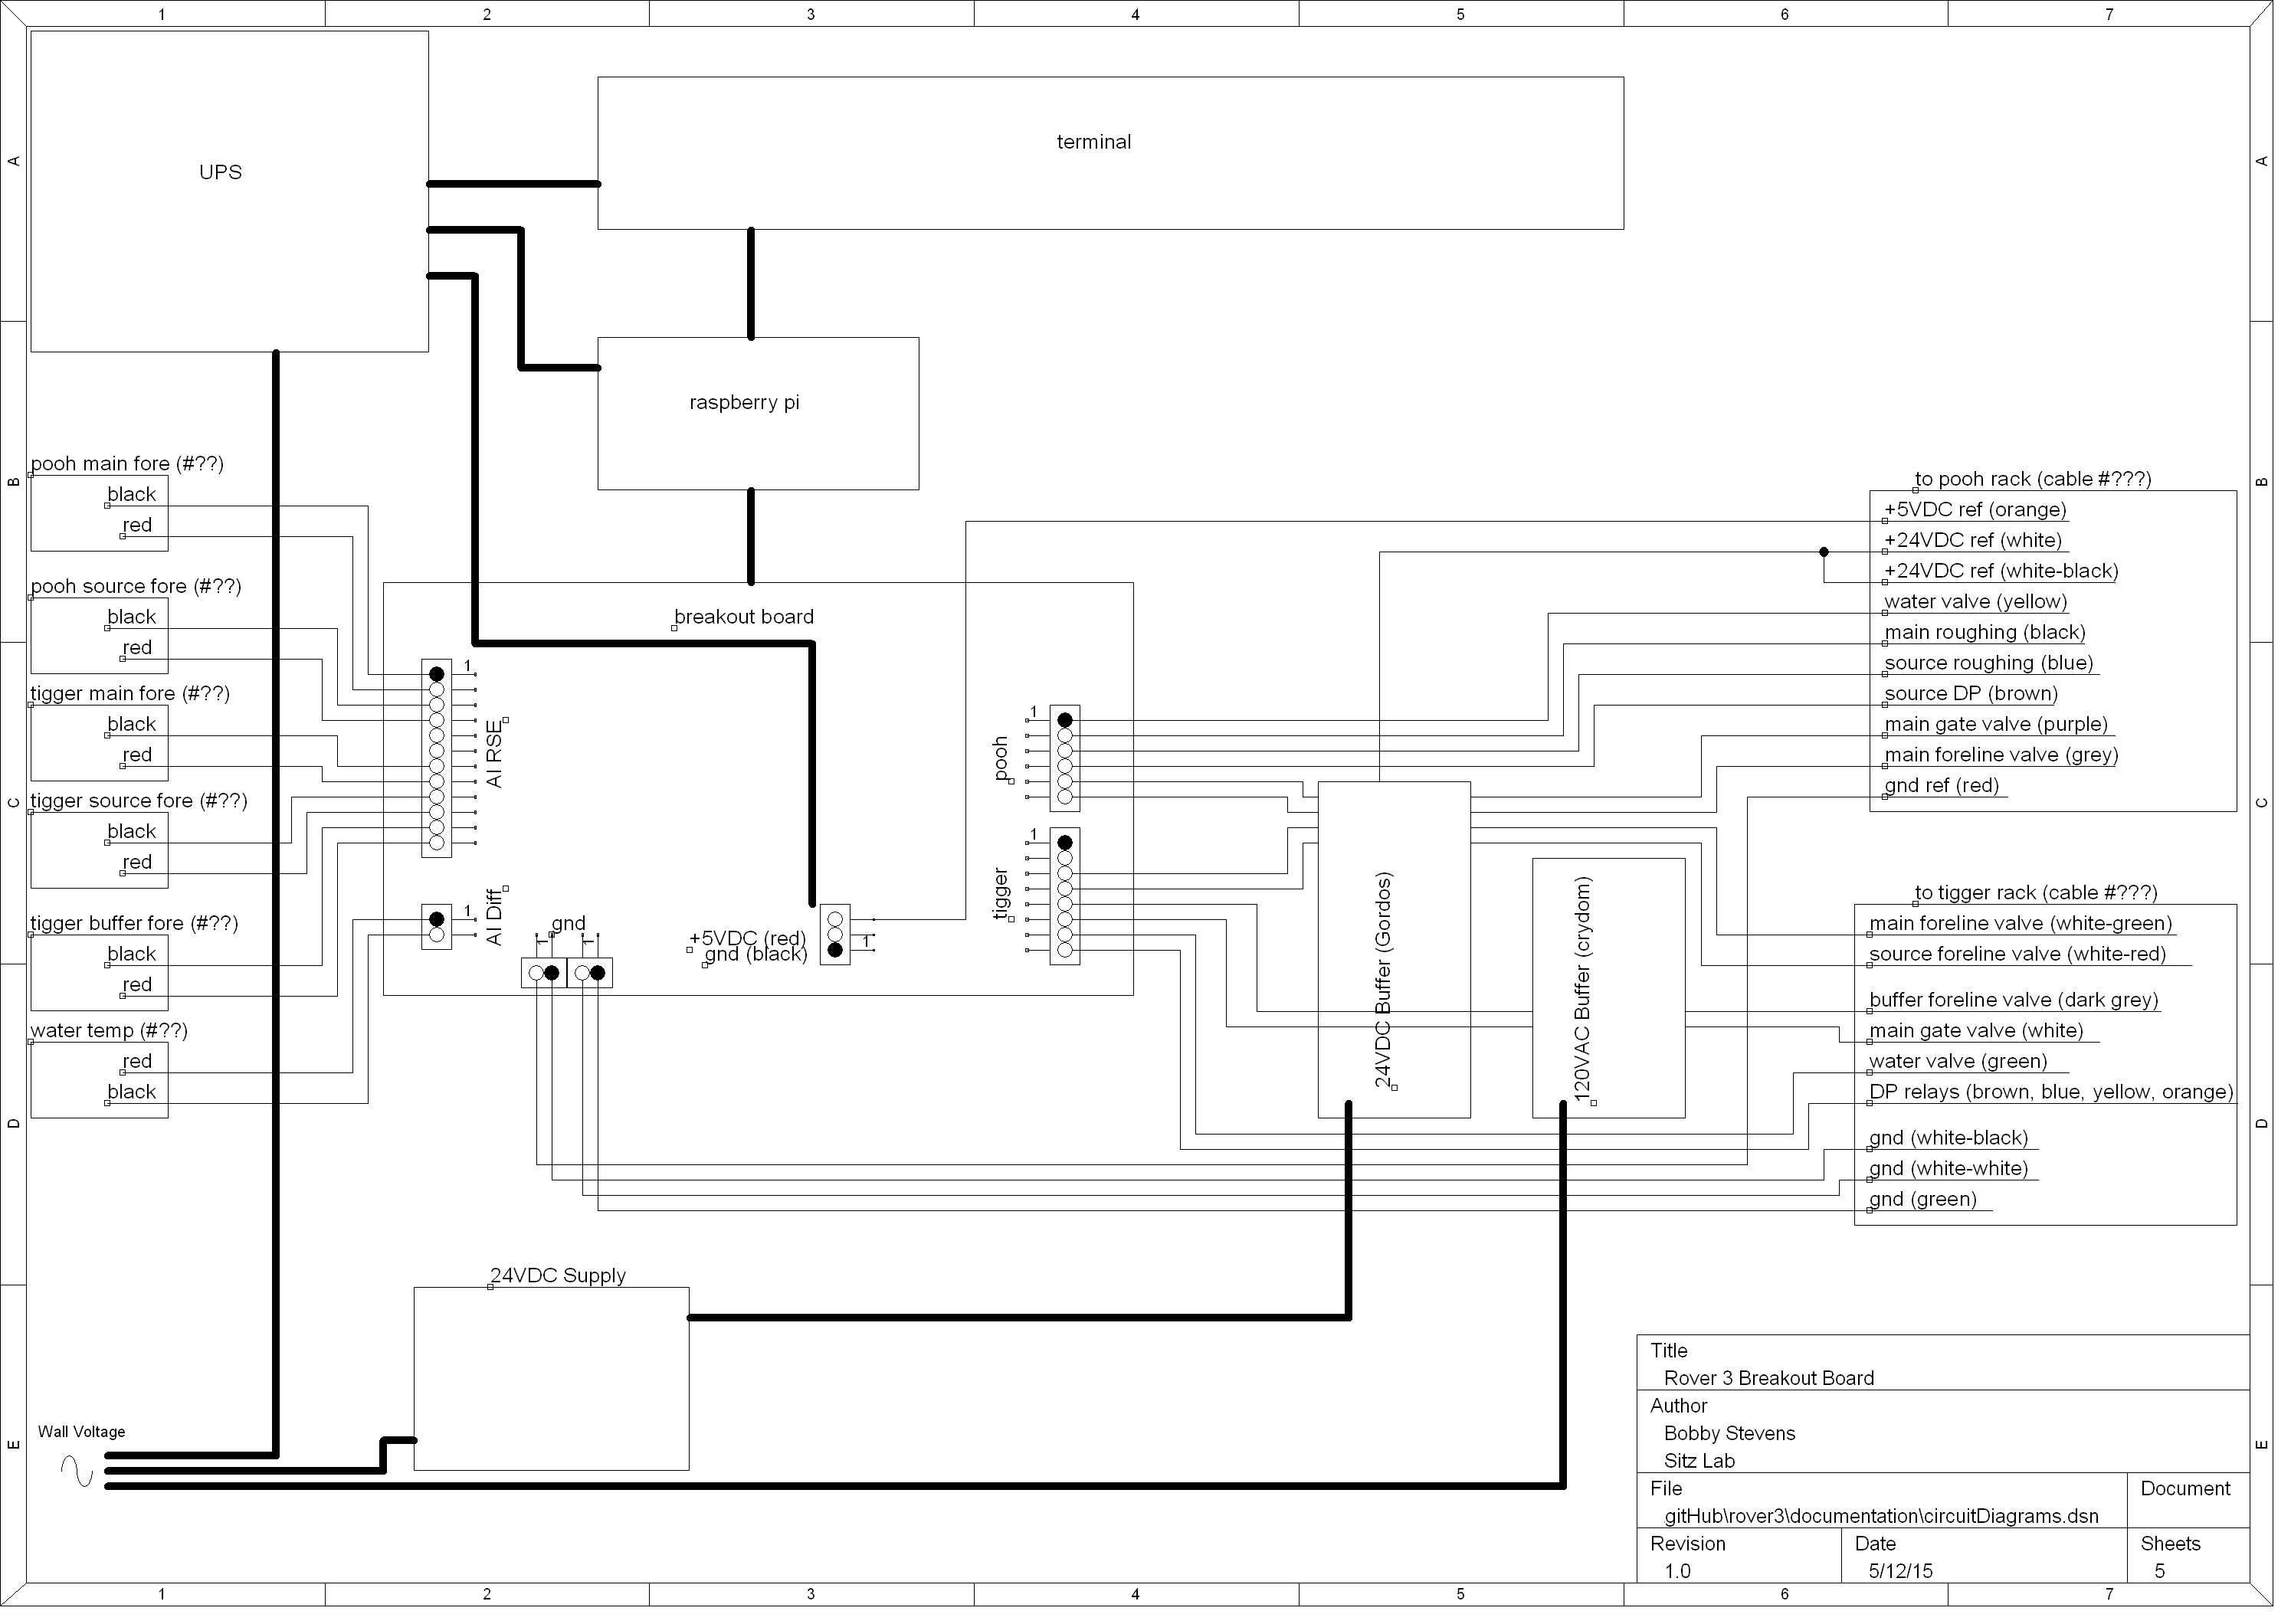
\includegraphics[width=0.9\textwidth]{wiringDiagram.png}
\caption{}
\label{fig:wiringDiagram}
\end{figure}



\section{Start Up \& Common Usage}

\subsection{Rebooting Rover}
At startup the RP2 will not automatically log in. So you must first login as \textbf{\texttt{students}} with the password \textbf{\texttt{scatter12}}. Then you must manually start the graphical enviroment with \textbf{\texttt{startx}}. Once it has finished loading the desktop open a terminal window (icon on top bar on the left side) and navigate to \url{cd ~\Desktop\Rover3\}. Run the Rover Server with super user access: \texttt{sudo python roverServer.py}. It will resume its last current configuration. You will see a window like figure \ref{fig:ssMain}.

\begin{figure}
\centering
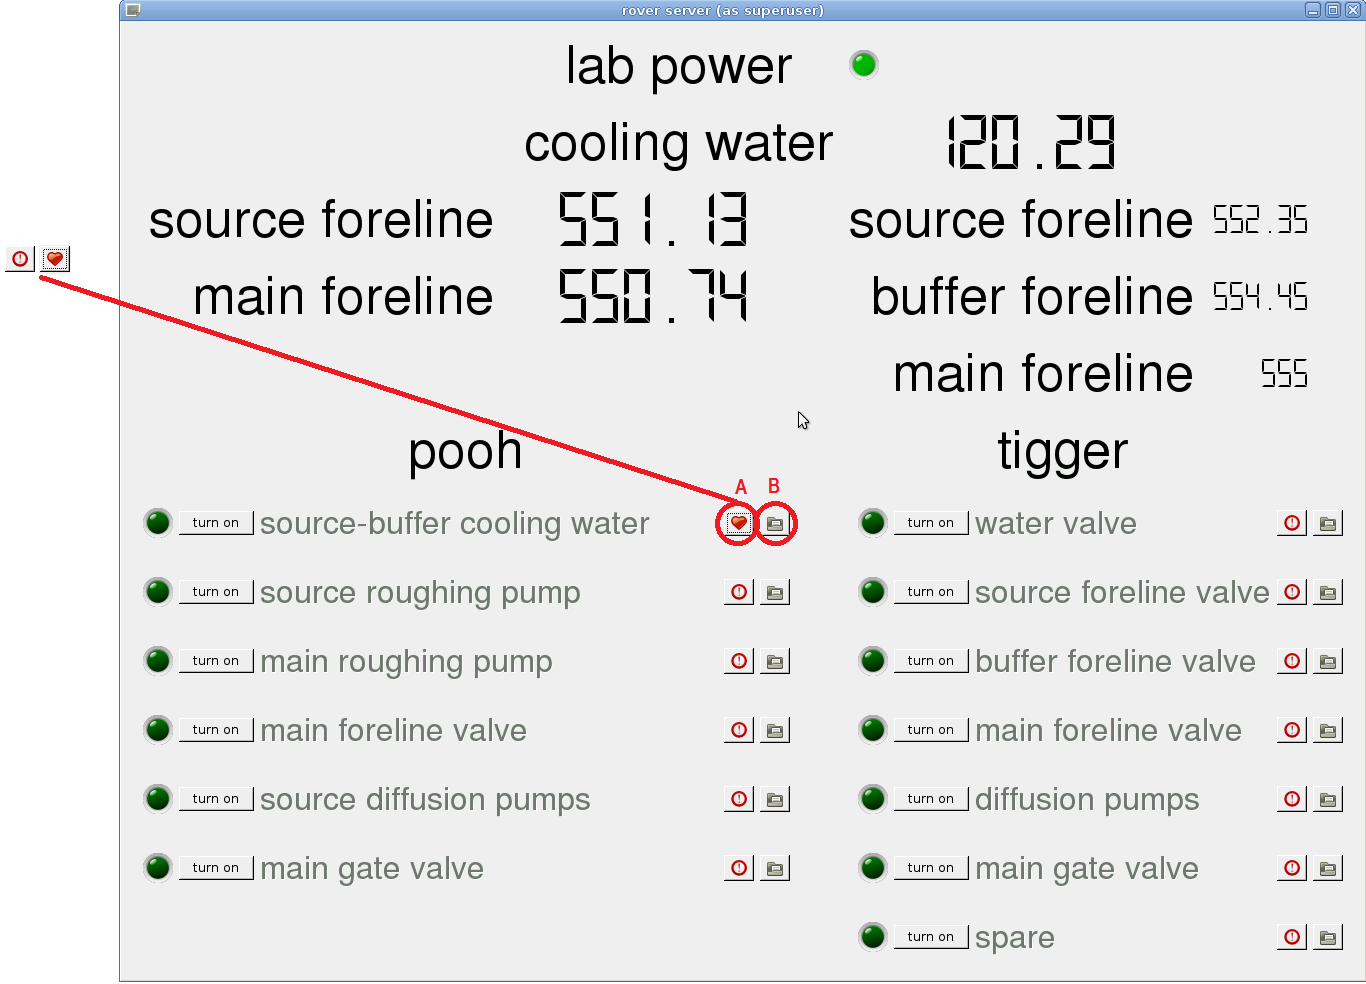
\includegraphics[width=0.9\textwidth]{ssMain.png}
\caption{The main interface window for Rover 3. Sensor inputs along the top are displayed in millivolts when in debug mode or milliTorr/degrees celcius when not. Each relay control has its own row in the bottom half. Button A is the interlock override with the inset displaying the interlocks disabled icon (exclaimation point) and enabled icon (heart). Button B is the interlock configuration button which will spawn the window displayed in figure \ref{fig:ssInter} and is used to configure interlocks for that relay.}
\label{fig:ssMain}
\end{figure}


\subsection{Programming Interlocks}
To program interlocks first click the interlock config button for the device you wish to control (figure \ref{fig:ssMain}) which will spawn the interlock config window, figure \ref{fig:ssInter}. Set up a new interlock by picking which sensor you want to monitor followed by the logical level you want this sensor to remain relative to the set point. \textbf{When this logical statement is \emph{true} the interlock will trip and turn the DOObject off.} To create the interlock click the add button on the left. To commit the shown interlocks click the okay button. The interlocks are written to a config file for each control object and will persist after restarting Rover.

\begin{figure}
\centering
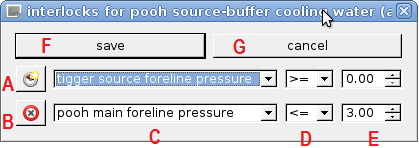
\includegraphics[width=0.9\textwidth]{ssInter.png}
\caption{The interlock configuration window for Rover 3. Button A will create the interlock displayed in the top row. Button B will delete the interlock on that row. Combo boxes and spinbox C, D, and E are the input sensor, logical level on which to trip, and set point respectively. Remember that \textbf{true} statements cause the interlock to trip and shut the relay off. Button F will commit the current changes and button G will discard them.}
\label{fig:ssInter}
\end{figure}

If a device's interlocks are tripping and you wish to override you can disable the enforcement of interlocks with the interlock override button, see figure \ref{fig:ssMain}. A heart indicates that interlocks are being enforced while a exclaimation point indicates they are not. After an interlock trips and turns the device off the interlocks will be overriden for that device. This means that if an interlock trips you can simply force the device on by clicking `turn on' once more.

\subsection{Recovery from Power Loss}
Should the lab lose power unexpectedly Rover will be aware of it. Rover senses the lab power through a voltage divider on the +24VDC supply which is plugged direction into the wall (\textbf{NOT the uninterruptable power supply}). Rover has been programmed that in the event of power loss it should turn every device off and not turn devices back on once lab power is restored. Since both the 24VDC and 120VAC ancillary boards are powered directly from the wall those devices will shut off as soon as power is lost while the other devices will remain on for the approximate half second it takes Rover to respond. 

Rover is powered through the uninterruptable power supply so it should be able to remain on for roughly 6 hours without any lab power. If the UPS runs out Rover will lose power as well. If you anticipate power to be out for longer than 6 hours you should shut Rover down so that a corruption of the file system is not a possibility.


\section{Troubleshooting Guide}
Here we will outline the basic problems and solutions that have been observed during design and assembly. This is by no means a complete guide but will cover the most likely to occur problems.
\newline
\newline

If you are having problems with Rover your first step should be to rerun roverServer in debug mode: \texttt{sudo python roverServer.py debug}. This will write all the log status to the terminal window and not the log file as well as display all sensor readings in millivolts.
\newline
\newline


\noindent
\textbf{Symptom: the AI channels all read the same and it doesn't update (eg. 24). This should also be accompanied with an message in the transcript file 'lost connection to ADCs! Retrying in .5s...'.}

\noindent
\textbf{Cause: connection with the ADC units has been compromised.}

\noindent
\textbf{\emph{Solution 0:}} Check the physical connection between the sensors and the screw terminals.

\noindent
\textbf{\emph{Solution 1:}} First check the ribbon cable connection between the RP2 and backplane board.

\noindent
\textbf{\emph{Solution 2:}} the 5VDC supply for the backplane may not be working. Check its voltage at the black 2-screw terminal in the lower right quadrant.

\noindent
\textbf{\emph{Solution 3:}} Attach a oscilloscope between TP2 and TP0 and between TP3 and TP0. Close RoverServer.py. Execute \texttt{sudo i2cdetect -y 1}. The scope should display 16-bit bursts on both channels (see figure \ref{fig:i2cTiming}). If the logic levels are not sharp edges there is stray capacitance somewhere on either the clock or data lines. This causes the I2C bus to not register the addresses properly. This will be further confirmed by the i2cdetect program not showing an entry for 0x63 or 0x64 (the addresses of the ADCs). First check the connection on R1 and R2. These are pull-up resistors that should improve this voltage timing. Next check the connections on the I2C clock and data wires coming from the RP2 breakout to the ADCs (orange and green).
\newline
\newline

\noindent
\textbf{Symptom: python error - maximum recursion depth exceeded}

\noindent
\textbf{Cause: this is an antiquated version of \texttt{roverServer.py} which uses a recursive function to poll the ADCs in a thread.}

\noindent
\textbf{\emph{Solution 0:}} Make sure that someone didn't accidentally revert back to this recursive function. The class that does the ADC acquisition in \texttt{roverServer.py} should be a subclass of thread and should not end with a call to itself.
\newline
\newline



\noindent
\textbf{Symptom: turning a relay off is not actually toggling the device}

\noindent
\textbf{Cause: the relay control line is not working. A few malfunctioning devices could be causing this.}

\noindent
\textbf{\emph{Solution 0:}} Check your connections to devices at the screw terminals. See figure \ref{fig:wiringDiagram}. If they are all connected proceed.

\noindent
\textbf{\emph{Solution 1:}} First check the ribbon cable connection between the RP2 and backplane board.

\noindent
\textbf{\emph{Solution 2:}} the 5VDC supply for the backplane may not be working. Check its voltage at the black 2-screw terminal in the lower right quadrant.

\noindent
\textbf{\emph{Solution 3:}} Attach a oscilloscope between TP1 and TP0. This will be observing the clock pin sent to the 574 chips. The 574 will only update its output to match its input when this pin is clocked low to high. Toggle a device in \texttt{roverServer.py}. Does the scope show a clocking event? If no, check the connection between RP2 GPIO pin \#4 and pin \#11 on each of the 574s. If that is connected, check the source code for \texttt{roverServer.py} and make sure there is a method defined \texttt{clockPin} and it is being sent to each \texttt{digitalOutput} object upon initialization. If the 574s are both being clocked and their outputs are indeed not updating then the chip is faulty and needs to be replaced.

\noindent
\textbf{\emph{Solution 4:}} If the problem is localized to the Crydom 120VAC relays make sure that you are connecting a load across the relay's AC terminals. These relays won't actually power unless it sees a load and a DVM doesn't count!

\end{document}
